\documentclass[aspectratio=169, 11pt]{beamer}

% Packages
\usepackage[utf8]{inputenc}
\usepackage{amsmath, amssymb, amsfonts}
\usepackage{graphicx}
\usepackage{booktabs}
\usepackage{ragged2e}
\usepackage{minted}
\usepackage{xcolor}
\usepackage{tikz}
\usepackage{algorithm}
\usepackage{algorithmic}
\usepackage{listings}
\usepackage{tikz}

\usetikzlibrary{arrows.meta,positioning,fit,shapes.symbols}
\usetikzlibrary{arrows,shapes}
\definecolor{LightGray}{gray}{0.975}
\definecolor{links}{HTML}{2A1B81}
\hypersetup{colorlinks,linkcolor=,urlcolor=blue}
\AtBeginEnvironment{minted}{%
    \renewcommand{\fcolorbox}[4][]{#4}
}

\title[Regression]{ML101 \\ Lecture 03: Linear Regression}
\subtitle{An Introduction to Statistical Learning}
\author{James, Witten, Hastie \& Tibshirani}
\date{\today}

% Remove navigation symbols...
\setbeamertemplate{navigation symbols}{}

\defbeamertemplate*{footline}{shadow theme}{
    \leavevmode
    \hbox{
        \begin{beamercolorbox}[
                wd =        0.33\paperwidth,
                ht =        2.5ex,
                dp =        1.125ex,
                leftskip =  0.3cm plus1fil,
                rightskip = 0.3cm
            ]{author in head/foot}
            \flushleft ML101
        \end{beamercolorbox}
        \begin{beamercolorbox}[
                wd =        0.33\paperwidth,
                ht =        2.5ex,
                dp =        1.125ex,
                leftskip =  0.3cm plus1fil,
                rightskip = 0.3cm
            ]{author in head/foot}
            \insertshorttitle
        \end{beamercolorbox}
        \begin{beamercolorbox}[
                wd =        0.33\paperwidth,
                ht =        2.5ex,
                dp =        1.125ex,
                leftskip =  0.3cm plus1fil,
                rightskip = 0.3cm
            ]{title in head/foot}
            \hfill \insertframenumber\,/\,\inserttotalframenumber%
        \end{beamercolorbox}
    }
}

\AtBeginSection[]
{
     \begin{frame}<beamer>
     \frametitle{Plan}
     \tableofcontents[currentsection]
     \end{frame}
}

\usefonttheme{serif}

\newcommand\Wider[2][18mm]{%
    \makebox[\linewidth][c]{%
        \begin{minipage}{\dimexpr\textwidth+#1\relax}
            \raggedright#2
        \end{minipage}%
    }%
}
\newcommand\userinput[1]{\textbf{#1}}

\begin{document}

\frame{\titlepage}

\begin{frame}{An Introduction to Statistical Learning with Applications in R}{a.k.a. ISLR}
    \centering
    
\includegraphics[height=0.75\textheight]{figures/book_cover} \\
    \vspace{2mm}
    {
        \tiny
        Content has been extracted from \textit{An Introduction to Statistical Learning with Applications in R}, Second Edition, by James, Witten, Hastie \& Tibshirani. Springer. 2023.\\
        Visit \url{https://www.statlearning.com/}.\\
    }
\end{frame}

\section{Simple Linear Regression}

\begin{frame}{Linear Regression}
  \begin{itemize}
    \item Linear regression is a simple approach to supervised learning. It assumes that the dependence of $Y$ on $X_1, X_2, \dots, X_p$ is linear.
    \item True regression functions are never linear!
    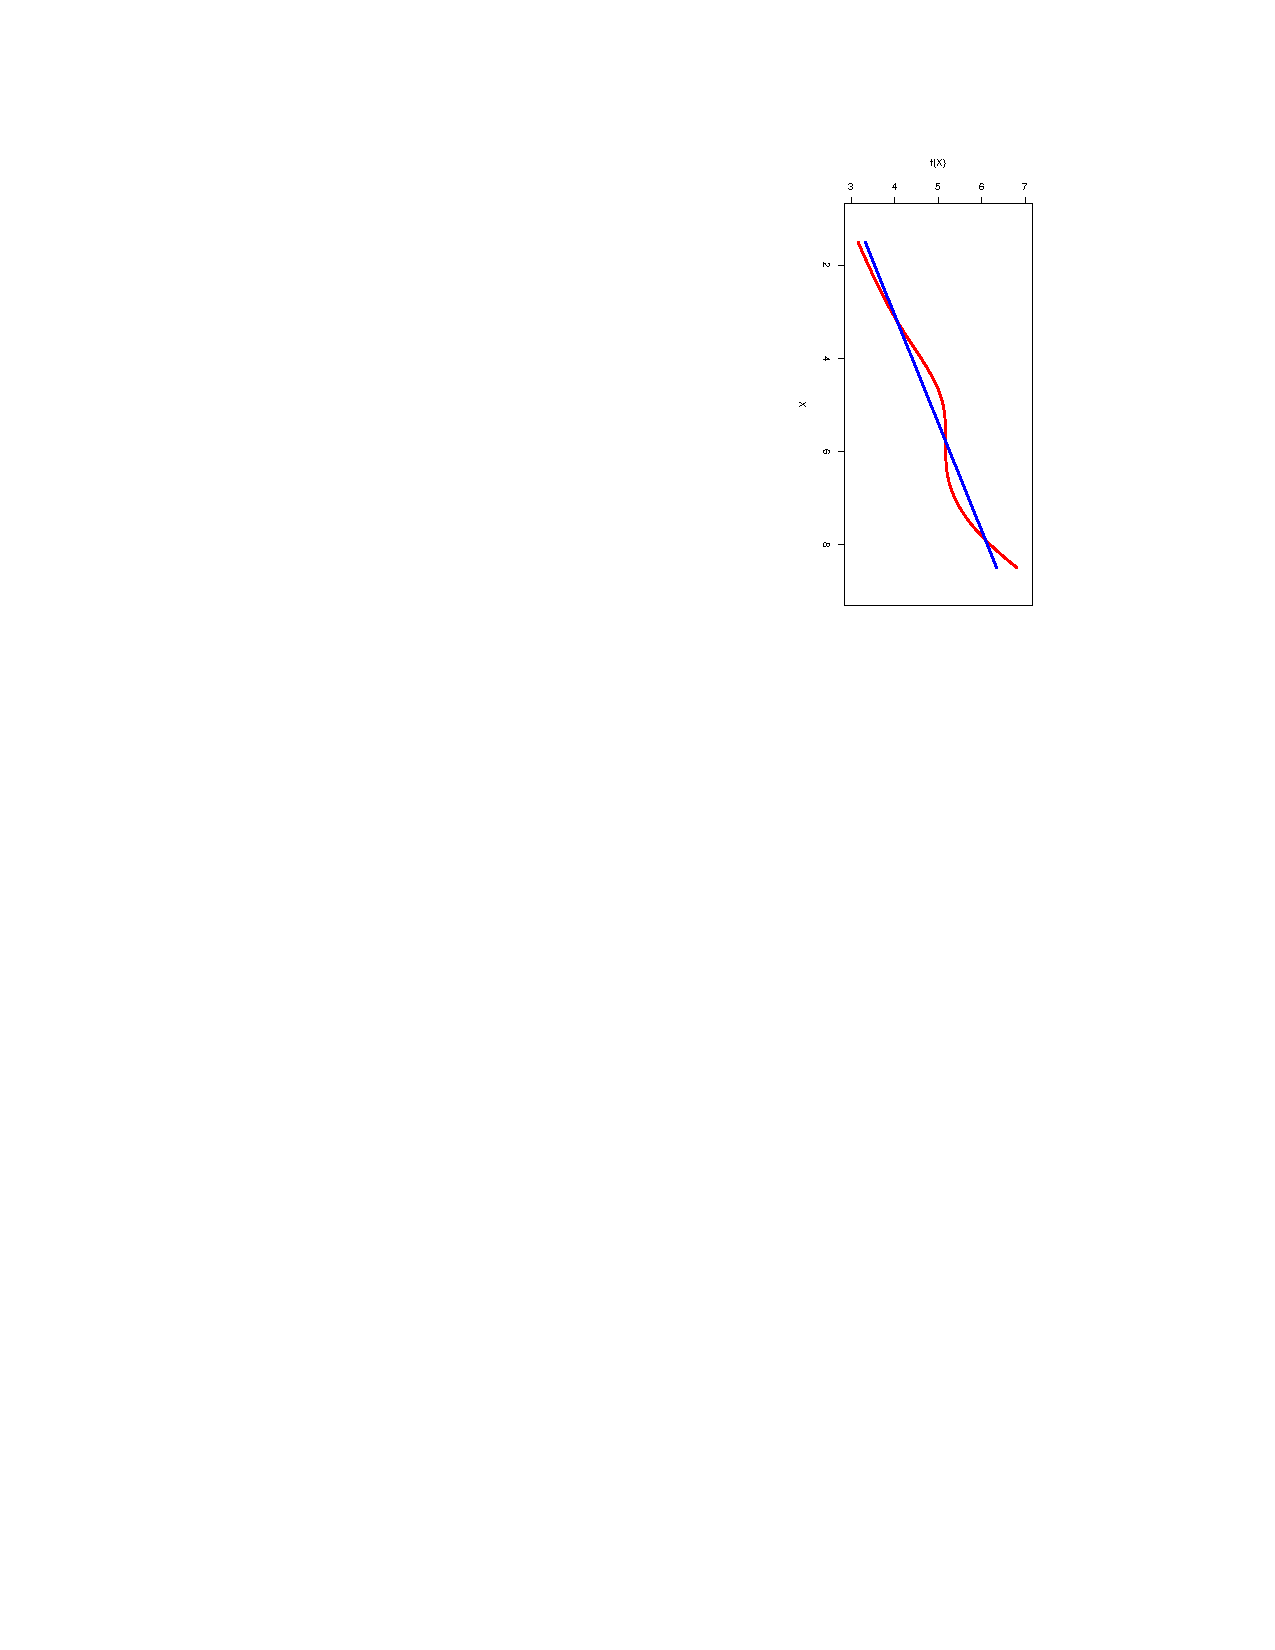
\includegraphics[angle=90, width=0.7\textwidth]{figures/01_lr} \pause
    \item Although it may seem overly simplistic, linear regression is extremely useful both conceptually and practically.
  \end{itemize}
\end{frame}

\begin{frame}{Linear Regression for the Advertising Data}
  Consider the advertising data. Questions we might ask:
  \begin{itemize}
    \item Is there a relationship between advertising budget and sales?
    \item How strong is the relationship between advertising budget and sales?
    \item Which media contribute to sales?
    \item How accurately can we predict future sales?
    \item Is the relationship linear?
    \item Is there synergy among the advertising media?
  \end{itemize}
\end{frame}

\begin{frame}{Advertising data}
  \centering
  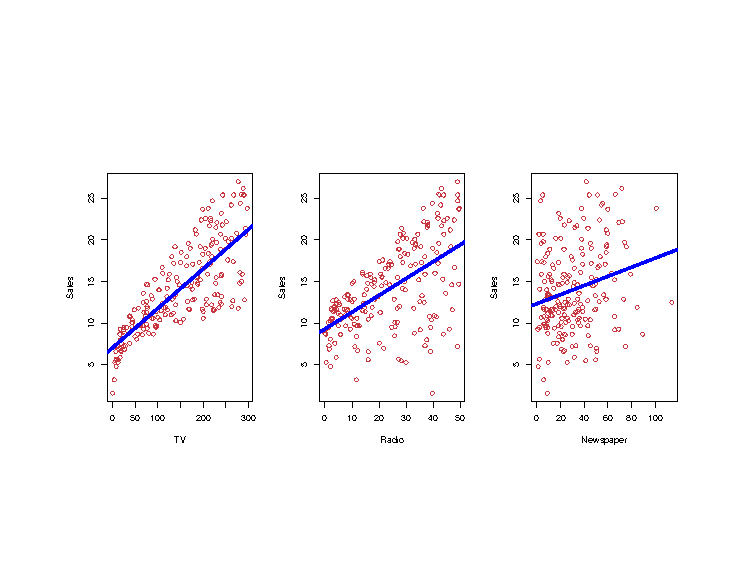
\includegraphics[width=\textwidth]{figures/ad}
\end{frame}

\begin{frame}{Simple Linear Regression}
  Simple linear regression using a single predictor $X$:
  \begin{itemize}
    \item We assume a model:
    \[ Y = \beta_0 + \beta_1 X + \epsilon \]
    where $\beta_0$ and $\beta_1$ are two unknown constants that represent the \textbf{intercept} and \textbf{slope}, also known as \textbf{coefficients} or \textbf{parameters}, and $\epsilon$ is the error term.
    
    \item Given some estimates $\hat{\beta}_0$ and $\hat{\beta}_1$ for the model coefficients, we predict future sales using:
    \[ \hat{y} = \hat{\beta}_0 + \hat{\beta}_1 x \]
    where $\hat{y}$ indicates a prediction of $Y$ on the basis of $X = x$. The \textbf{hat} symbol denotes an estimated value.
  \end{itemize}
\end{frame}

\subsection{Estimating the Coefficients}

\begin{frame}{Estimation of the Parameters by Least Squares}
  \begin{itemize}
    \item Let $\hat{y}_i = \hat{\beta}_0 + \hat{\beta}_1 x_i$ be the prediction for $Y$ based on the $i$-th value of $X$. Then $e_i = y_i - \hat{y}_i$ represents the $i$-th \textbf{residual}.
    \item We define the \textbf{residual sum of squares} (RSS) as:
    \[ RSS = e_1^2 + e_2^2 + \dots + e_n^2 \]
    or equivalently as:
    \[ RSS = (y_1 - \hat{\beta}_0 - \hat{\beta}_1 x_1)^2 + (y_2 - \hat{\beta}_0 - \hat{\beta}_1 x_2)^2 + \dots + (y_n - \hat{\beta}_0 - \hat{\beta}_1 x_n)^2 \]
    \item The least squares approach chooses $\hat{\beta}_0$ and $\hat{\beta}_1$ to minimize the RSS. The minimizing values are:
    \[ \hat{\beta}_1 = \frac{\sum_{i=1}^n (x_i - \bar{x})(y_i - \bar{y})}{\sum_{i=1}^n (x_i - \bar{x})^2}, \quad \hat{\beta}_0 = \bar{y} - \hat{\beta}_1 \bar{x} \]
    where $\bar{y} \equiv \frac{1}{n} \sum_{i=1}^n y_i$ and $\bar{x} \equiv \frac{1}{n} \sum_{i=1}^n x_i$ are the sample means.
  \end{itemize}
\end{frame}

\begin{frame}{Example: advertising data}
  \centering
  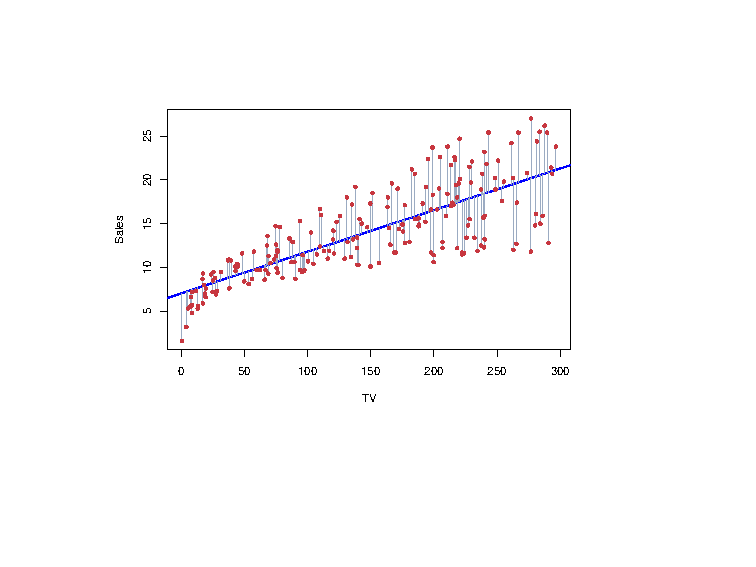
\includegraphics[width=0.7\textwidth]{figures/ad2} \\
  The least squares fit for the regression of \texttt{sales} and \texttt{TV}.  In this case a linear fit captures the essence of the relationship, although it is somewhat deficient in the left of the plot.
\end{frame}

\subsection{Assessing the Accuracy of the Coefficient Estimates}

\begin{frame}{Assessing the Accuracy of the Coefficient Estimates}
  \begin{itemize}
    \item The standard error of an estimator reflects how it varies under repeated sampling:
    \[ SE(\hat{\beta}_1)^2 = \frac{\sigma^2}{\sum_{i=1}^n (x_i - \bar{x})^2}, \quad SE(\hat{\beta}_0)^2 = \sigma^2 \left[ \frac{1}{n} + \frac{\bar{x}^2}{\sum_{i=1}^n (x_i - \bar{x})^2} \right] \]
    where $\sigma^2 = \text{Var}(\epsilon)$. \pause
    
    \item These standard errors can be used to compute \textbf{confidence intervals}. A 95\% confidence interval is defined as a range of values such that with 95\% probability, the range will contain the true unknown value of the parameter. It has the form:
    \[ \hat{\beta}_1 \pm 2 \cdot SE(\hat{\beta}_1) \]
  \end{itemize}
\end{frame}

% Frame 6
\begin{frame}{Confidence Intervals Continued}
  \begin{itemize}
    \item That is, there is approximately a 95\% chance that the interval:
    \[ [\hat{\beta}_1 - 2 \cdot SE(\hat{\beta}_1), \, \hat{\beta}_1 + 2 \cdot SE(\hat{\beta}_1)] \]
    will contain the true value of $\beta_1$ (under a scenario where we got repeated samples like the present sample). \pause
    \item For the advertising data, the 95\% confidence interval for $\beta_1$ is $[0.042, 0.053]$.
  \end{itemize}
\end{frame}

% Frame 7
\begin{frame}{Hypothesis Testing}
  \begin{itemize}
    \item Standard errors can also be used to perform \textbf{hypothesis tests} on the coefficients. The most common hypothesis test involves testing the \textbf{null hypothesis} of:
    \begin{align*}
      H_0 :& \text{There is no relationship between } X \text{ and } Y \\
           & \text{versus the \textbf{alternative hypothesis}} \\
      H_A :& \text{There is some relationship between } X \text{ and } Y\text{.}
    \end{align*}
    \pause
    \item Mathematically, this corresponds to testing:
    \[ H_0: \beta_1 = 0 \quad \text{versus} \quad H_A: \beta_1 \neq 0 \]
    since if $\beta_1 = 0$ then the model reduces to $Y = \beta_0 + \epsilon$, and $X$ is not associated with $Y$.
  \end{itemize}
\end{frame}

% Frame 8
\begin{frame}{Hypothesis Testing -- continued}
  \begin{itemize}
    \item To test the null hypothesis, we compute a \textcolor{orange}{\textit{t-statistic}}, given by:
    \[ t = \frac{\hat{\beta}_1 - 0}{SE(\hat{\beta}_1)} \]
    \item This will have a $t$-distribution with $n-2$ degrees of freedom, assuming $\beta_1 = 0$.
    \item Using statistical software, it is easy to compute the probability of observing any value equal to $|t|$ or larger. We call this probability the \textcolor{orange}{\textit{p-value}}.
  \end{itemize}
\end{frame}

% Frame 9
\begin{frame}{Results for the Advertising Data}
  \begin{table}
    \centering
    \begin{tabular}{l c c c c}
      \toprule
      & \textbf{Coefficient} & \textbf{Std. Error} & \textbf{$t$-statistic} & \textbf{$p$-value} \\
      \midrule
      \textbf{Intercept} & 7.0325 & 0.4578 & 15.36 & $<$ 0.0001 \\
      \textbf{TV}        & 0.0475 & 0.0027 & 17.67 & $<$ 0.0001 \\
      \bottomrule
    \end{tabular}
  \end{table}
\end{frame}

% Frame 10
\begin{frame}{Assessing the Overall Accuracy of the Model}
  \begin{itemize}
    \item We compute the \textbf{Residual Standard Error}:
    \[
      RSE = \sqrt{\frac{1}{n-2} RSS} = \sqrt{\frac{1}{n-2} \sum_{i=1}^n (y_i - \hat{y}_i)^2},
    \]
    where the \textbf{residual sum-of-squares} is $RSS=\sum_{i=1}^n (y_i - \hat{y}_i)^2$. \pause
    \item \textbf{R-squared} or fraction of variance explained is:
    \[ R^2 = \frac{TSS - RSS}{TSS} = 1 - \frac{RSS}{TSS} \]
    where $TSS = \sum_{i=1}^n (y_i - \bar{y})^2$ is the \textbf{total sum of squares}. \pause
    \item In simple linear regression, $R^2 = r^2$, where $r$ is the sample correlation between $X$ and $Y$:
    \[ r = \frac{\sum_{i=1}^n (x_i - \bar{x})(y_i - \bar{y})}{\sqrt{\sum_{i=1}^n (x_i - \bar{x})^2} \sqrt{\sum_{i=1}^n (y_i - \bar{y})^2}} \]
  \end{itemize}
\end{frame}

\subsection{Assessing the Accuracy of the Model}

\begin{frame}{Advertising Data Results}
  \begin{table}
    \centering
    \begin{tabular}{l c}
      \toprule
      \textbf{Quantity} & \textbf{Value} \\
      \midrule
      Residual Standard Error & 3.26 \\
      $R^2$                   & 0.612 \\
      $F$-statistic           & 312.1 \\
      \bottomrule
    \end{tabular}
  \end{table}
\end{frame}

\section{Multiple Linear Regression}

\begin{frame}{Multiple Linear Regression}
  \begin{itemize}
    \item Here our model is:
    \[ Y = \beta_0 + \beta_1 X_1 + \beta_2 X_2 + \dots + \beta_p X_p + \epsilon \]
    \item We interpret $\beta_j$ as the \textbf{average} effect on $Y$ of a one unit increase in $X_j$, \textbf{holding all other predictors fixed}. In the advertising example, the model becomes:
    \[ \text{\texttt{sales}} = \beta_0 + \beta_1 \times \text{\texttt{TV}} + \beta_2 \times \text{\texttt{radio}} + \beta_3 \times \text{\texttt{newspaper}} + \epsilon \]
  \end{itemize}
\end{frame}

% Frame 13
\begin{frame}{Interpreting Regression Coefficients}
  \begin{itemize}
    \item The ideal scenario is when the predictors are uncorrelated -- a \textbf{balanced design}:
    \begin{itemize}
      \item Each coefficient can be estimated and tested separately.
      \item Interpretations such as \textit{``a unit change in $X_j$ is associated with a $\beta_j$ change in $Y$, while all other variables stay fixed''}, are possible.
    \end{itemize}
    \item Correlations amongst predictors cause problems:
    \begin{itemize}
      \item The variance of all coefficients tends to increase, sometimes dramatically.
      \item Interpretations become hazardous: when $X_j$ changes, everything else changes.
    \end{itemize}
    \item \textbf{Claims of causality} should be avoided for observational data.
  \end{itemize}
\end{frame}

% Frame 14
\begin{frame}{The Woes of (Interpreting) Regression Coefficients}
  \begin{quote}
    ``Data Analysis and Regression'' -- Mosteller and Tukey (1977)
  \end{quote}
  A regression coefficient $\beta_j$ estimates the expected change in $Y$ per unit change in $X_j$, \textbf{with all other predictors held fixed}. But predictors usually change together! \pause
  
  \begin{itemize}
    \item \textbf{Example 1:} $Y = \text{total change in pocket}$; $X_1 = \text{\# of coins}$; $X_2 = \text{\# of pennies, nickels, dimes}$. By itself, coefficient of $Y$ on $X_2$ is $> 0$. But with $X_1$ in the model? \pause

    \item \textbf{Example 2:} $Y = \text{number of tackles by a football player in a season}$; $W$ and $H$ are his weight and height. Fitted regression model is $\hat{Y} = b_0 + 0.50 W - 0.10 H$. How do we interpret $\hat{\beta}_2 < 0$?
  \end{itemize}
\end{frame}

% Frame 15
\begin{frame}{Two Quotes by Famous Statisticians}
  \begin{block}{George Box}
    ``Essentially, all models are wrong, but some are useful.''
  \end{block}
  \pause
  \vspace{0.5cm}
  \begin{block}{Fred Mosteller and John Tukey (paraphrasing George Box)}
    ``The only way to find out what will happen when a complex system is disturbed is to disturb the system, not merely to observe it passively.''
  \end{block}
\end{frame}

\subsection{Estimating the Regression Coefficients}

\begin{frame}{Estimation and Prediction for Multiple Regression}
  \begin{itemize}
    \item Given estimates $\hat{\beta}_0, \hat{\beta}_1, \dots, \hat{\beta}_p$, we can make prediction using the formula:
    \[ \hat{y} = \hat{\beta}_0 + \hat{\beta}_1 x_1 + \hat{\beta}_2 x_2 + \dots + \hat{\beta}_p x_p \]
    \item We estimate $\hat{\beta}_0, \hat{\beta}_1, \dots, \hat{\beta}_p$ as the values that minimize the sum of squared residuals:
    \[ RSS = \sum_{i=1}^n (y_i - \hat{y}_i)^2 = \sum_{i=1}^n (y_i - \hat{\beta}_0 - \hat{\beta}_1 x_{i1} - \dots - \hat{\beta}_p x_{ip})^2 \]
    This is done using standard statistical software.  The values $\hat{\beta}_0, \hat{\beta}_1, \dots, \hat{\beta}_p$ that minimize RSS are the multiple least squares regression estimates.
  \end{itemize}
\end{frame}

\begin{frame}{}
  \centering
  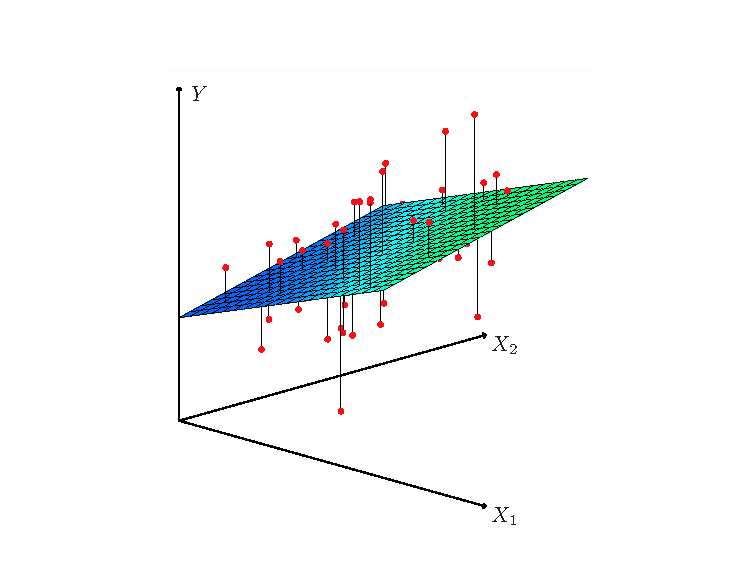
\includegraphics[height=0.9\textheight]{figures/plane01}
\end{frame}

\begin{frame}{Results for Advertising Data}
  \begin{table}
    \centering
    \begin{tabular}{l c c c c}
      \toprule
      & \textbf{Coefficient} & \textbf{Std. Error} & \textbf{$t$-statistic} & \textbf{$p$-value} \\
      \midrule
      \textbf{Intercept} & 2.939  & 0.3119 & 9.42   & $<$0.0001 \\
      \textbf{TV}        & 0.046  & 0.0014 & 32.81  & $<$0.0001 \\
      \textbf{radio}     & 0.189  & 0.0086 & 21.89  & $<$0.0001 \\
      \textbf{newspaper}& -0.001 & 0.0059 & -0.18  & 0.8599  \\
      \bottomrule
    \end{tabular}
  \end{table}

  \vspace{0.2cm}
  \textbf{Correlations:}
  \begin{table}
    \centering
    \small
    \begin{tabular}{l c c c c}
      \toprule
      & \textbf{TV} & \textbf{radio} & \textbf{newspaper} & \textbf{sales} \\
      \midrule
      \textbf{TV}        & 1.0000 & 0.0548 & 0.0567 & 0.7822 \\
      \textbf{radio}     &        & 1.0000 & 0.3541 & 0.5762 \\
      \textbf{newspaper} &        &        & 1.0000 & 0.2283 \\
      \textbf{sales}     &        &        &        & 1.0000 \\
      \bottomrule
    \end{tabular}
  \end{table}
\end{frame}

\subsection{Some Important Questions}

\begin{frame}{Some Important Questions}
  \begin{enumerate}
    \item Is at least one of the predictors $X_1, X_2, \dots, X_p$ useful in predicting the response? \pause
    \item Do all the predictors help to explain $Y$, or is only a subset of the predictors useful? \pause
    \item How well does the model fit the data? \pause
    \item Given a set of predictor values, what response value should we predict, and how accurate is our prediction? \pause
  \end{enumerate}
\end{frame}

\begin{frame}{Is at Least One Predictor Useful?}
  For the first question, we can use the $F$-statistic:
  \[ F = \frac{\frac{(TSS - RSS)}{p}}{\frac{RSS}{n - p - 1}} \sim F_{p, \, n-p-1} \]

  \begin{table}
    \centering
    \begin{tabular}{l c}
      \toprule
      \textbf{Quantity} & \textbf{Value} \\
      \midrule
      Residual Standard Error & 1.69 \\
      $R^2$                   & 0.897 \\
      $F$-statistic           & 570 \\
      \bottomrule
    \end{tabular}
  \end{table}
\end{frame}

% Frame 20
\begin{frame}{Deciding on the Important Variables}
  \begin{itemize}
    \item \textbf{All Subsets / Best Subsets Regression:} Compute least squares fit for all possible subsets and choose based on a criterion balancing training error and model size. \pause
    \item However, there are $2^p$ possible models (e.g., $p=40 \implies >1$ billion models!).
    \item Instead we need an automated approach that searches through a subset of them.  The book discusses two commonly use approaches next.
  \end{itemize}
\end{frame}

% Frame 21
\begin{frame}{Variable Selection Methods}
  \begin{block}{Forward Selection}
    \begin{itemize}
      \item Begin with the \textbf{null model} (a model that contains an intercept but no predictors).
      \item Fit $p$ simple linear regression and add to the null model the variable that results in the lowest RSS.
      \item Add to that model the variable that results in the lowest RSS amongst all two-variable models.
      \item Continue adding variables one by one until a stopping rule is satisfied. i.e. when all remaining variables have a \textit{p-value} above some threshold.
    \end{itemize}
  \end{block}
\end{frame}

\begin{frame}{Variable Selection Methods}
  \begin{block}{Backward Selection}
    \begin{itemize}
      \item Start with all variables in the model.
      \item Remove the variable with the largest \textit{p-value} (that is, the variable that is the least statistically significant).
      \item The new $(p-1)$-variable model is fit, and the variable with the largest \textit{p-value} is removed.
      \item Continue until a stopping rule is reached.  i.e. we may stop when all remaining variable have a significant \textit{p-value} defined by some significance threshold.
    \end{itemize}
  \end{block}
\end{frame}

\begin{frame}{Model Selection Criteria}
  Other systematic criteria for choosing an optimal model path include:
  \begin{itemize}
    \item Mallow's $C_p$
    \item Akaike Information Criterion (AIC)
    \item Bayesian Information Criterion (BIC)
    \item Adjusted $R^2$
    \item Cross-Validation (CV)
  \end{itemize}
\end{frame}

\section{Other Considerations in the Regression Model}

\subsection{Qualitative Predictors}

\begin{frame}{Qualitative Predictors}
  \begin{itemize}
    \item Qualitative predictors take a discrete set of values (also known as \textbf{categorical} predictors or \textbf{factor variables}).
    \item i.e. In addition to the 7 quantitative variables shown, there are four qualitative variables: \texttt{gender}, \texttt{student} (student status), \texttt{status} (marital status), and \texttt{ethnicity} (Caucasian, African American or Asian).
  \end{itemize}
\end{frame}

\begin{frame}{Credit card data}
  \centering
  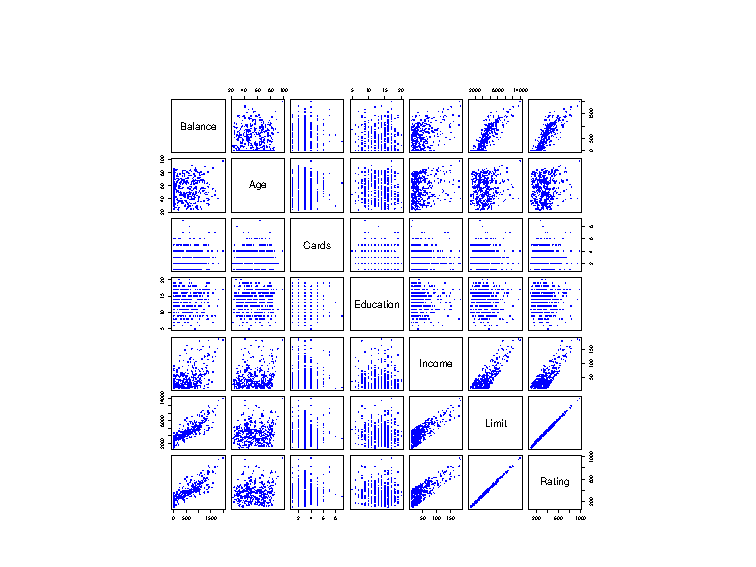
\includegraphics[height=0.93\textheight]{figures/sp}
\end{frame}

\begin{frame}{Qualitative Predictors --continued}
  \begin{itemize}
    \item Example: investigate differences in credit card balance between males and females, ignoring the other variables.
    \item We create a new variable (a binary predictor, e.g. gender: Female/Male):
    \[ x_i = \begin{cases} 1 & \text{if } i\text{-th person is female} \\ 0 & \text{if } i\text{-th person is male} \end{cases} \]
    \item Resulting model:
    \[ y_i = \beta_0 + \beta_1 x_i + \epsilon_i = \begin{cases} \beta_0 + \beta_1 + \epsilon_i & \text{if female} \\ \beta_0 + \epsilon_i & \text{if male} \end{cases} \] \pause
    \item Interpretation?
  \end{itemize}
\end{frame}

\begin{frame}{Credit card data --continued}
  Results for gender model:
  \begin{table}
    \centering
    \begin{tabular}{l c c c c}
      \toprule
      & \textbf{Coefficient} & \textbf{Std. Error} & \textbf{$t$-statistic} & \textbf{$p$-value} \\
      \midrule
      \textbf{Intercept}      & 509.80 & 33.13 & 15.389 & $<$0.0001 \\
      \textbf{gender[Female]} &  19.73 & 46.05 &  0.429 &    0.6690 \\
      \bottomrule
    \end{tabular}
  \end{table}
\end{frame}

\begin{frame}{Qualitative Predictors with More Than Two Levels}
  \begin{itemize}
    \item With $k > 2$ levels, create $k-1$ dummy variables.
    \item i.e. for \textbf{ethnicity} (Asian, Caucasian, African American) create two dummy variables:
    \[ x_{i1} = \begin{cases} 1 & \text{if Asian} \\ 0 & \text{otherwise} \end{cases}, \quad x_{i2} = \begin{cases} 1 & \text{if Caucasian} \\ 0 & \text{otherwise} \end{cases} \]
    \item Resulting model:
    \[ y_i = \beta_0 + \beta_1 x_{i1} + \beta_2 x_{i2} + \epsilon_i = \begin{cases} \beta_0 + \beta_1 + \epsilon_i & \text{if Asian} \\ \beta_0 + \beta_2 + \epsilon_i & \text{if Caucasian} \\ \beta_0 + \epsilon_i & \text{if African American (baseline)} \end{cases} \]
  \end{itemize}
\end{frame}

\begin{frame}{Qualitative Predictors with More Than Two Levels --continued}
  \begin{itemize}
    \item Then both of these variables can be used in the regression equation, in order to obtain the model:
    \[ y_i = \beta_0 + \beta_1 x_{i1} + \beta_2 x_{i2} + \epsilon_i = \begin{cases} \beta_0 + \beta_1 + \epsilon_i & \text{if Asian} \\ \beta_0 + \beta_2 + \epsilon_i & \text{if Caucasian} \\ \beta_0 + \epsilon_i & \text{if African American (baseline)} \end{cases} \]
  \end{itemize}
  \vspace{15mm}
  {\small \textbf{Note}: There will always be one fewer dummy variable than the number of levels.  The level with no dummy variable --AA in this example-- is known as the \textbf{baseline}}
\end{frame}

\begin{frame}{Results for \texttt{ethnicity}}
  \begin{table}
    \centering
    \begin{tabular}{l c c c c}
      \toprule
      & \textbf{Coefficient} & \textbf{Std. Error} & \textbf{$t$-statistic} & \textbf{$p$-value} \\
      \midrule
      \textbf{Intercept}            & 531.00 & 46.32 & 11.464 & $<$0.0001 \\
      \textbf{ethnicity[Asian]}     & -18.69 & 65.02 & -0.287 &    0.7740 \\
      \textbf{ethnicity[Caucasian]} & -12.50 & 56.68 & -0.221 &    0.8260 \\
      \bottomrule
    \end{tabular}
  \end{table}
\end{frame}

\subsection{Extensions of the Linear Model}

\begin{frame}{Extensions of the Linear Model}
  Removing the additive assumption: \textit{interactions} and \textit{nonlinearity}...
  \begin{itemize}
    \item \textbf{Interactions}:
      \begin{itemize}
        \item In our previous analysis of the \texttt{Advertising} data, we assumed that the effect on \texttt{sales} of increasing one advertising medium is independent of the amount spent on the other media.

        \item i.e. the linear model:
          \[ \text{sales} = \beta_0 + \beta_1 \times \text{TV} + \beta_2 \times \text{radio} + \beta_3 \times \text{newspaper} \]
        states that the average effect on \texttt{sales} of a one-unit increase in TV is always $\beta_1$, regardless of the amount spent on \texttt{radio}.
    \end{itemize}
  \end{itemize}
\end{frame}

\begin{frame}{Extensions of the Linear Model --continued}
  \begin{itemize}
    \item \textbf{Interactions}:
    \begin{itemize}
      \item But suppose that spending money on radio advertising actually increases the effectiveness of TV advertising, so that the slope term for \texttt{TV} should increase as \texttt{radio} increases.
      \item In this situation, given a fixed budget of \$100,000, spending half on \texttt{radio} and half on \texttt{TV} may increase \texttt{sales} more than allocating the entire amount to either \texttt{TV} or to \texttt{radio}.
      \item In marketing, this is known as a \textbf{synergy} effect, and in statistics it is referred to as an \textbf{interaction} effect.
    \end{itemize}
  \end{itemize}
\end{frame}

\begin{frame}{Interaction in the Advertising data?}
  \centering
  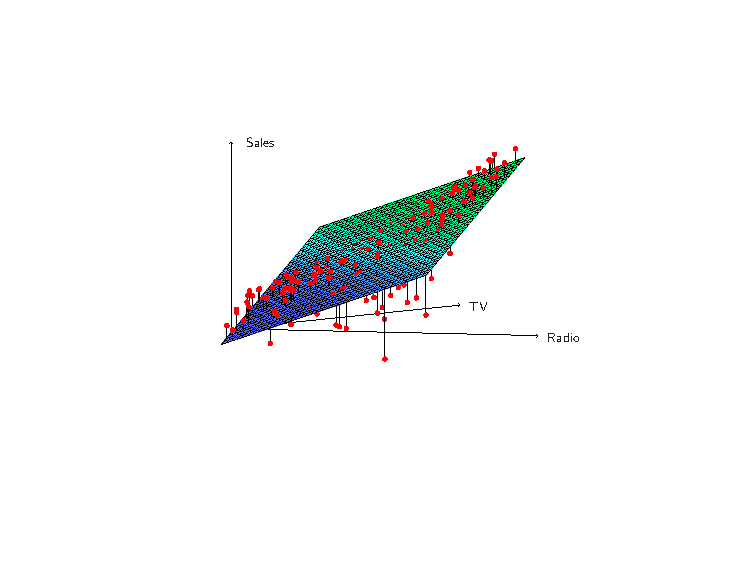
\includegraphics[width=0.6\textwidth]{figures/p36}
  \begin{itemize}
    \item When levels of either \texttt{TV} or \texttt{radio} are low, then the true \texttt{sales} are lower than predicted by the linear model.
    \item But when advertising is split between the two media, then the model tends to understimate \texttt{sales}.
  \end{itemize}

\end{frame}

\begin{frame}{Modelling Interactions -- Advertising Data Results}
  Model takes the form:
  \begin{align*}
    \text{sales} &= \beta_0 + \beta_1 \times \text{TV} + \beta_2 \times \text{radio} + \beta_3 \times (\text{TV} \times \text{radio}) + \epsilon \\
    &= \beta_0 + (\beta_1 + \beta_3 \times \text{radio}) \times \text{TV} + \beta_2 \times \text{radio} + \epsilon
  \end{align*}
  \begin{table}
    \centering
    \begin{tabular}{l c c c c}
      \toprule
      & \textbf{Coefficient} & \textbf{Std. Error} & \textbf{$t$-statistic} & \textbf{$p$-value} \\
      \midrule
      \textbf{Intercept}  & 6.7502  & 0.2480  & 27.23 & $< 0.0001$ \\
      \textbf{TV}         & 0.0191  & 0.0015  & 12.70 & $< 0.0001$ \\
      \textbf{radio}      & 0.0289  & 0.0089  & 3.24  & 0.0014     \\
      \textbf{TV$\times$radio} & 0.0011 & 0.0001 & 20.73 & $< 0.0001$ \\
      \bottomrule
    \end{tabular}
  \end{table}
\end{frame}

\begin{frame}{Interpretation}
  \begin{itemize}
    \item The results in this table suggests that interactions are important.
    \item The \textit{p-value} for the interaction term \texttt{TV} $\times$ \texttt{radio} is extremely low, indicating that there is strong evidence for $H_A : \beta_3 \neq 0$.
    \item $R^2$ increases from 89.7\% (additive) to 96.8\% (with interaction).
  \end{itemize}
\end{frame}

\begin{frame}{Interpretation --continued}
  \begin{itemize}
    \item Explains variability remaining after fitting additive model!

    \item This means that
      $$\frac{96.8 - 89.7}{100 - 89.7}=69\%$$
    of the variability in \texttt{sales} that remains after fitting the additive model has been explained by the interaction term.

    \item The coefficient estimates in the table suggest that an increase in TV advertising of \$1,000 is associated with increased sales of
      $$ (\hat{\beta}_1 + \hat{\beta}_3 \times \text{\texttt{radio}}) \times 1000 = 19 + 1.1 \times \text{\texttt{radio} units.} $$

    \item An increase in radio advertising of \$1,000 will be associated with an increase in sales of
      $$ (\hat{\beta}_1 + \hat{\beta}_3 \times \text{\texttt{TV}}) \times 1000 = 29 + 1.1 \times \text{\texttt{TV} units.} $$
  \end{itemize}
\end{frame}

\begin{frame}{The Hierarchy Principle}
  \begin{itemize}
    \item Sometimes it is the case that an interaction term has a very small \textit{p-value}, but the associated main effects (in this case, \texttt{TV} and \texttt{radio}) do not.
  \end{itemize}

  \begin{block}{Hierarchy Principle}
    \textit{If we include an interaction in a model, we should also include the main effects, even if the $p$-values associated with their coefficients are not significant.}
  \end{block}
\end{frame}

\begin{frame}{The Hierarchy Principle --continued}
  \begin{itemize}
    \item The rationale for this principle is that interactions are hard to interpret in a model without main effects --their meaning is changed.

    \item Specifically, the interaction terms also contain main effects, if the model has no main effect terms.
  \end{itemize}
\end{frame}

\begin{frame}{Interactions between qualitative and quantitative variables}
  \begin{itemize}
    \item Consider the \texttt{Credit} data set, and suppose that we wish to predict \texttt{balance} using \texttt{income} (quantitative) and \texttt{student} (qualitative).

    \item Without an interaction term, the model takes the form:
      \begin{align*}
        \text{\texttt{balance}}_i & \approx \beta_0 + \beta_1 \times  \text{\texttt{income}}_i + \begin{cases} \beta_2 & \text{if } i\text{-th person is a student} \\ 0 & \text{if } i\text{-th person is not a student} \end{cases} \\
                                  & = \beta_ \times \text{\texttt{income}}_i + \begin{cases} \beta_0 + \beta_2 & \text{if } i\text{-th person is a student} \\ \beta_0 & \text{if } i\text{-th person is not a student} \end{cases}
      \end{align*}
  \end{itemize}
\end{frame}

\begin{frame}{Interactions between qualitative and quantitative variables --continued}
  \begin{itemize}
    \item With interactions, it takes the form:
      \begin{align*}
        \text{\texttt{balance}}_i & \approx \beta_0 + \beta_1 \times  \text{\texttt{income}}_i +
          \begin{cases}
            \beta_2 + \beta_3 \times \text{\texttt{income}}_i & \text{if student} \\
            0 & \text{if not student}
          \end{cases} \\
          & =
            \begin{cases}
              (\beta_0 + \beta_2) + (\beta_1 + \beta_3) \times \text{\texttt{income}}_i & \text{if student} \\
              \beta_0 + \beta_1 \times \text{\texttt{income}}_i & \text{if not student}
            \end{cases}
      \end{align*}
  \end{itemize}
\end{frame}

\begin{frame}{Interactions between qualitative and quantitative variables --continued}
  \centering
  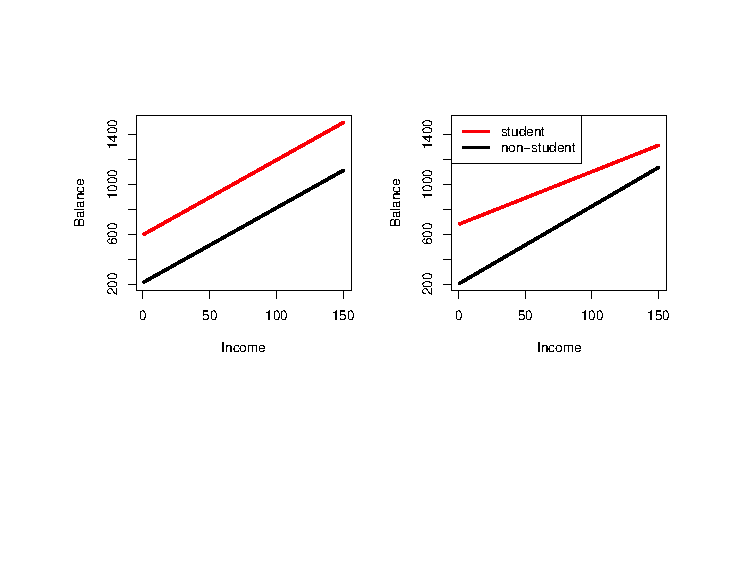
\includegraphics[width=0.90\textwidth]{figures/p44}
  \begin{itemize}
    \item Credit data; Left: no interaction between \texttt{income} and \texttt{student}. \\ Right: with an interaction term between \texttt{income} and \texttt{student}.
  \end{itemize}
\end{frame}

\begin{frame}{Non-linear Effects of Predictors}{polynomial regression on \texttt{Auto} data}
  \centering
  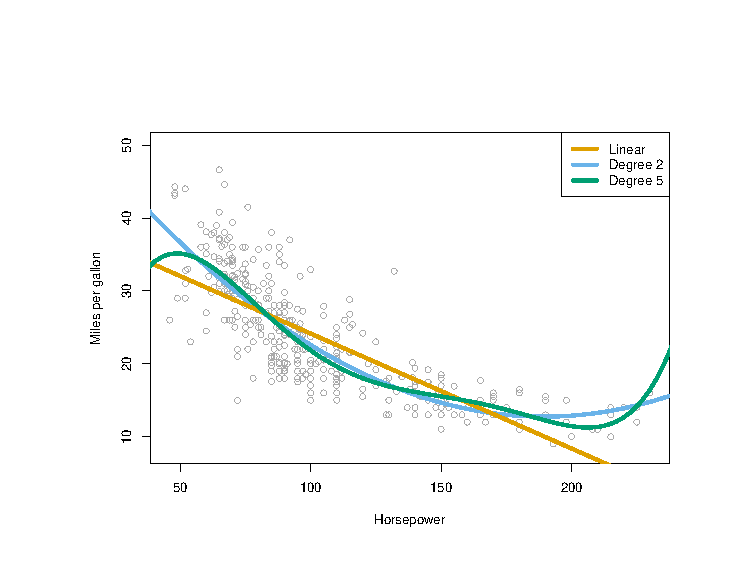
\includegraphics[width=0.75\textwidth]{figures/p45}
\end{frame}

\begin{frame}{Non-linear Effects of Predictors --continued}
  \begin{itemize}
    \item Polynomial Regression extends linear models to non-linear relationships.
    \item The figure suggests that:
    \[ \text{\texttt{mpg}} = \beta_0 + \beta_1 \times \text{\texttt{horsepower}} + \beta_2 \times \text{\texttt{horsepower}}^2 + \epsilon \]
  \end{itemize}

  \begin{table}
    \centering
    \begin{tabular}{l c c c c}
      \toprule
      & \textbf{Coefficient} & \textbf{Std. Error} & \textbf{$t$-statistic} & \textbf{$p$-value} \\
      \midrule
      \textbf{Intercept}      & 56.9001 & 1.8004 & 31.6  & $<$0.0001 \\
      \textbf{horsepower}     & -0.4662 & 0.0311 & -15.0 & $<$0.0001 \\
      \textbf{horsepower$^2$} & 0.0012  & 0.0001 & 10.1  & $<$0.0001 \\
      \bottomrule
    \end{tabular}
  \end{table}
\end{frame}

\subsection{Potential Problems}

\begin{frame}{What We Did Not Cover \& Generalizations}
  \begin{block}{Potential Issues in Regression (Section 3.3.3)}
    Outliers, Non-constant variance of error terms, High leverage points, Collinearity.
  \end{block}

  \begin{block}{Generalizations of the Linear Model}
    \begin{itemize}
      \item \textbf{Classification:} Logistic regression, Support Vector Machines.
      \item \textbf{Non-linearity:} Kernel smoothing, Splines, GAMs, Nearest Neighbors.
      \item \textbf{Interactions:} Tree-based methods, Bagging, Random Forests, Boosting (these also capture non-linearities).
      \item \textbf{Regularized fitting:} Ridge regression, Lasso
    \end{itemize}
  \end{block}
\end{frame}

\begin{frame}{}
     \centering
     \Huge End of Chapter 3.
\end{frame}

\begin{frame}{An Introduction to Statistical Learning with Applications in R}{a.k.a. ISLR}
    \centering
    
\includegraphics[height=0.75\textheight]{figures/book_cover} \\
    \vspace{2mm}
    {
        \tiny
        Content has been extracted from \textit{An Introduction to Statistical Learning with Applications in R}, Second Edition, by James, Witten, Hastie \& Tibshirani. Springer. 2023.\\
        Visit \url{https://www.statlearning.com/}.\\
    }
\end{frame}

\end{document}
